\documentclass[11pt]{article}
\usepackage[textwidth=18.0cm, textheight=23.0cm, top=2.0cm]{geometry}
\usepackage{pst-all}
\usepackage{amssymb}
\usepackage{tikz}
\usepackage{underscore}\begin{document}
\pagestyle{empty}


ClassName: \underline{\textbf{Class_07.2bp-12}}
\par
BinSize: \underline{\textbf{100 × 100}}
\par
ReduceSize: \underline{\textbf{100 × 100}}
\par
TypeNum: \underline{\textbf{40}}
\par
Num: \underline{\textbf{40}}
\par
OutS: \underline{\textbf{100000}}
\par
InS: \underline{\textbf{83209}}
\par
Rate: \underline{\textbf{0.832}}
\par
UB: \underline{\textbf{10}}
\par
LB0: \underline{\textbf{9}}
\par
LB: \underline{\textbf{10}}
\par
LBWithCut: \underline{\textbf{10}}
\par
NodeCut: \underline{\textbf{0}}
\par
ExtendedNodeCnt: \underline{\textbf{1}}
\par
GenNodeCnt: \underline{\textbf{1}}
\par
PrimalNode: \underline{\textbf{0}}
\par
ColumnCount: \underline{\textbf{121}}
\par
TotalCutCount: \underline{\textbf{0}}
\par
RootCutCount: \underline{\textbf{0}}
\par
LPSolverCnt: \underline{\textbf{112}}
\par
PricingSolverCnt: \underline{\textbf{112}}
\par
BranchAndBoundNum: \underline{\textbf{1}}
\par
isOpt: \underline{\textbf{true}}
\par
TimeOnPrimal: \underline{\textbf{0.000 s}}
\par
TimeOnPricing: \underline{\textbf{18.766 s}}
\par
TimeOnRmp: \underline{\textbf{0.105 s}}
\par
TotalTime: \underline{\textbf{18.954 s}}
\par
\newpage


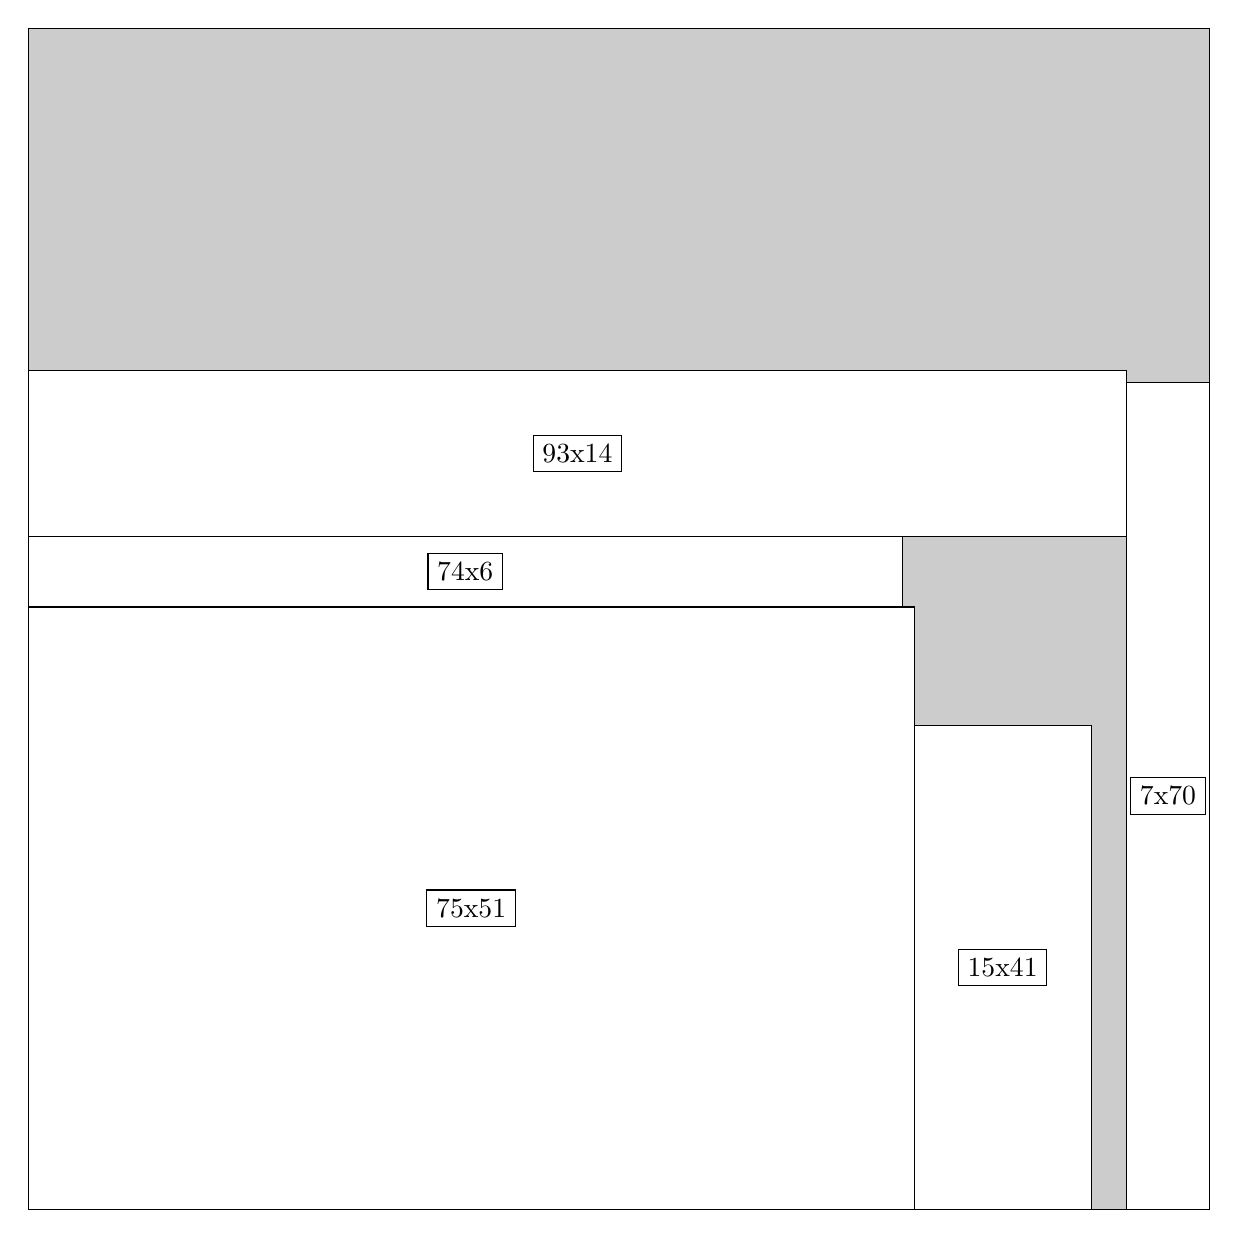
\begin{tikzpicture}[shorten >=1pt,scale=1.0,every node/.style={scale=1.0},->]
\tikzstyle{vertex}=[circle,fill=black!25,minimum size=14pt,inner sep=0pt]
\filldraw[fill=gray!40!white, draw=black] (0,0) rectangle (15.0,15.0);
\foreach \name/\x/\y/\w/\h in {75x51/0.0/0.0/11.25/7.6499999999999995,74x6/0.0/7.6499999999999995/11.1/0.8999999999999999,15x41/11.25/0.0/2.25/6.1499999999999995,7x70/13.95/0.0/1.05/10.5,93x14/0.0/8.549999999999999/13.95/2.1}
\filldraw[fill=white!40!white, draw=black] (\x,\y) rectangle node[draw] (\name) {\name} ++(\w,\h);
\end{tikzpicture}


w =75 , h =51 , x =0 , y =0 , v =3825
\par
w =74 , h =6 , x =0 , y =51 , v =444
\par
w =15 , h =41 , x =75 , y =0 , v =615
\par
w =7 , h =70 , x =93 , y =0 , v =490
\par
w =93 , h =14 , x =0 , y =57 , v =1302
\par
\newpage


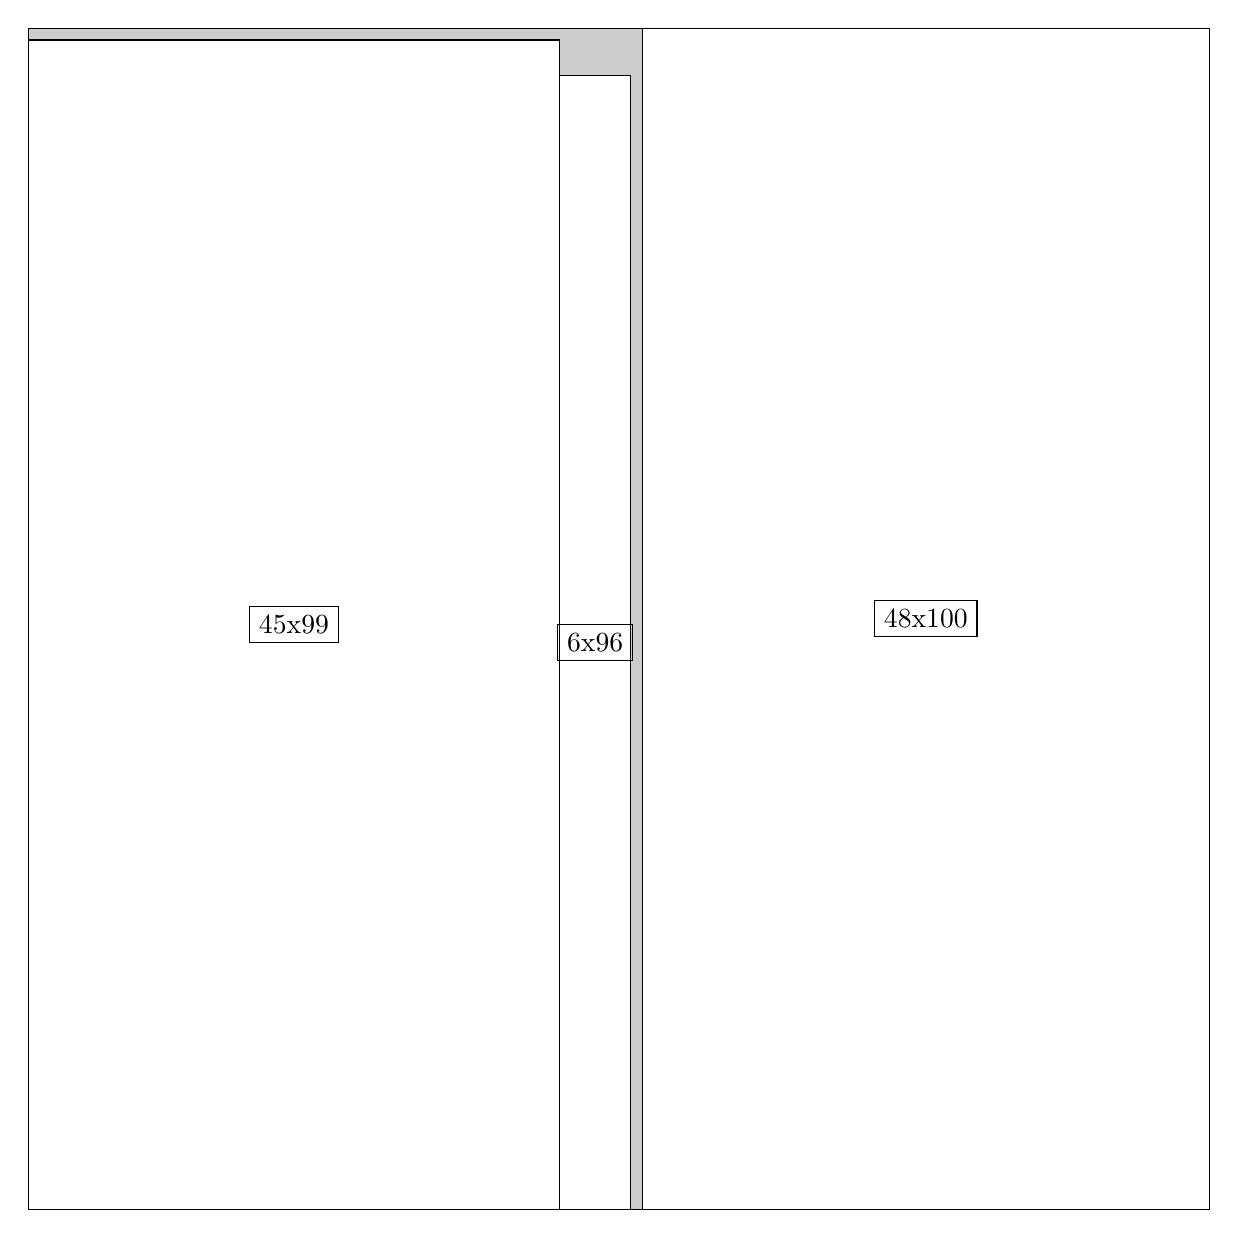
\begin{tikzpicture}[shorten >=1pt,scale=1.0,every node/.style={scale=1.0},->]
\tikzstyle{vertex}=[circle,fill=black!25,minimum size=14pt,inner sep=0pt]
\filldraw[fill=gray!40!white, draw=black] (0,0) rectangle (15.0,15.0);
\foreach \name/\x/\y/\w/\h in {48x100/7.8/0.0/7.199999999999999/15.0,45x99/0.0/0.0/6.75/14.85,6x96/6.75/0.0/0.8999999999999999/14.399999999999999}
\filldraw[fill=white!40!white, draw=black] (\x,\y) rectangle node[draw] (\name) {\name} ++(\w,\h);
\end{tikzpicture}


w =48 , h =100 , x =52 , y =0 , v =4800
\par
w =45 , h =99 , x =0 , y =0 , v =4455
\par
w =6 , h =96 , x =45 , y =0 , v =576
\par
\newpage


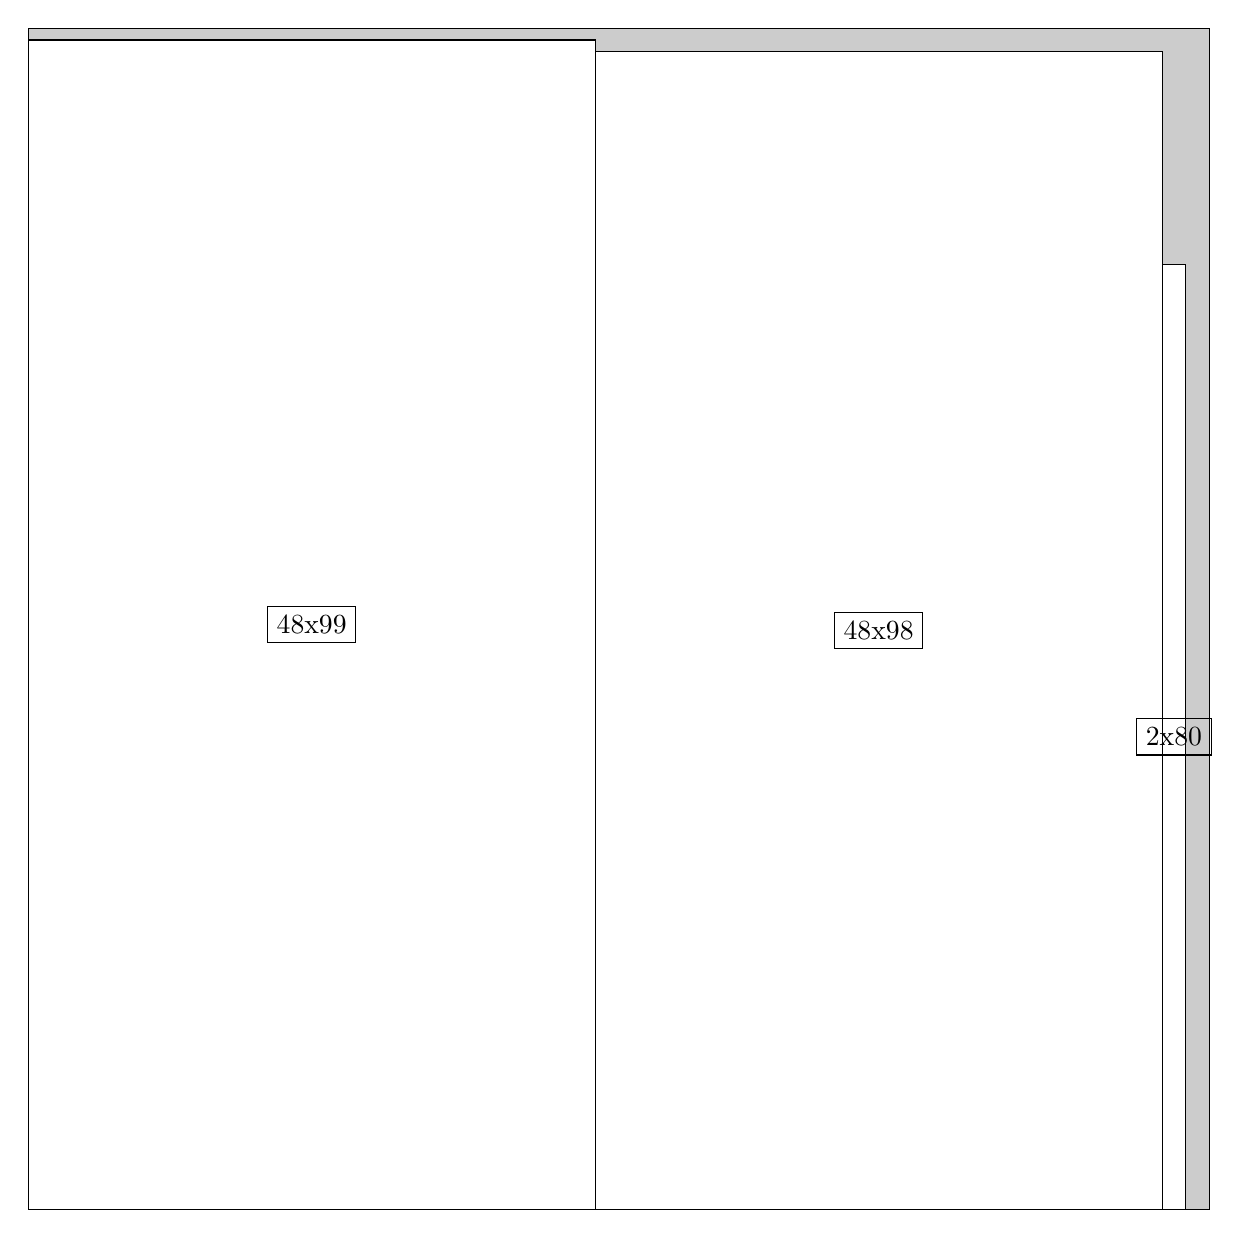
\begin{tikzpicture}[shorten >=1pt,scale=1.0,every node/.style={scale=1.0},->]
\tikzstyle{vertex}=[circle,fill=black!25,minimum size=14pt,inner sep=0pt]
\filldraw[fill=gray!40!white, draw=black] (0,0) rectangle (15.0,15.0);
\foreach \name/\x/\y/\w/\h in {48x99/0.0/0.0/7.199999999999999/14.85,48x98/7.199999999999999/0.0/7.199999999999999/14.7,2x80/14.399999999999999/0.0/0.3/12.0}
\filldraw[fill=white!40!white, draw=black] (\x,\y) rectangle node[draw] (\name) {\name} ++(\w,\h);
\end{tikzpicture}


w =48 , h =99 , x =0 , y =0 , v =4752
\par
w =48 , h =98 , x =48 , y =0 , v =4704
\par
w =2 , h =80 , x =96 , y =0 , v =160
\par
\newpage


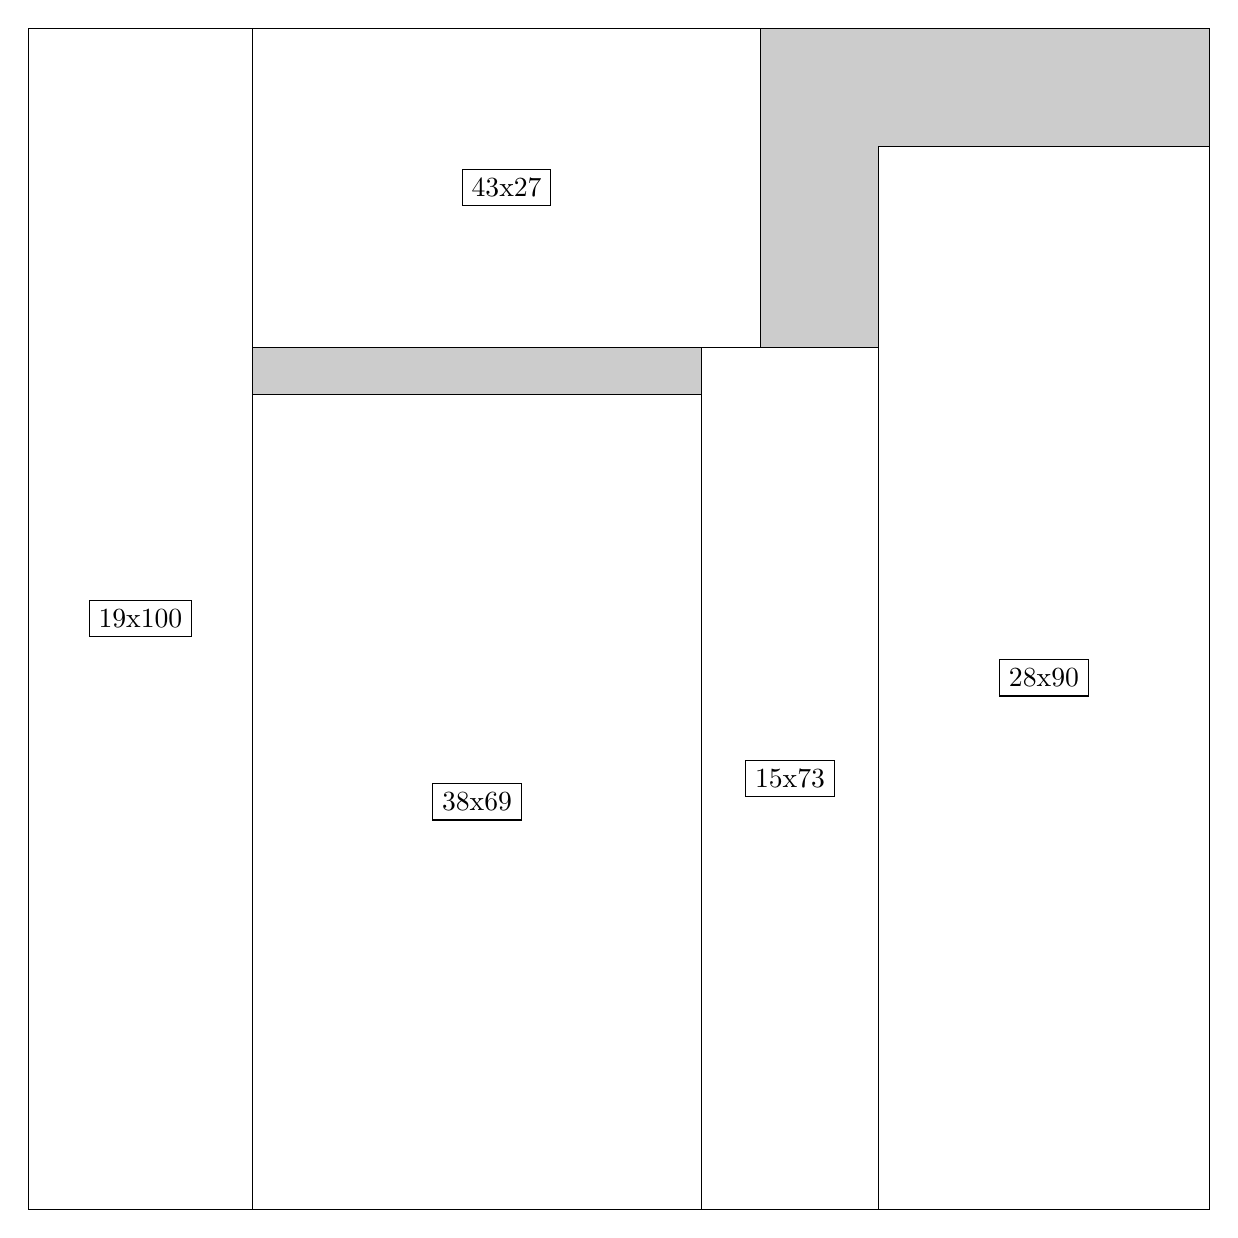
\begin{tikzpicture}[shorten >=1pt,scale=1.0,every node/.style={scale=1.0},->]
\tikzstyle{vertex}=[circle,fill=black!25,minimum size=14pt,inner sep=0pt]
\filldraw[fill=gray!40!white, draw=black] (0,0) rectangle (15.0,15.0);
\foreach \name/\x/\y/\w/\h in {38x69/2.85/0.0/5.7/10.35,28x90/10.799999999999999/0.0/4.2/13.5,19x100/0.0/0.0/2.85/15.0,43x27/2.85/10.95/6.45/4.05,15x73/8.549999999999999/0.0/2.25/10.95}
\filldraw[fill=white!40!white, draw=black] (\x,\y) rectangle node[draw] (\name) {\name} ++(\w,\h);
\end{tikzpicture}


w =38 , h =69 , x =19 , y =0 , v =2622
\par
w =28 , h =90 , x =72 , y =0 , v =2520
\par
w =19 , h =100 , x =0 , y =0 , v =1900
\par
w =43 , h =27 , x =19 , y =73 , v =1161
\par
w =15 , h =73 , x =57 , y =0 , v =1095
\par
\newpage


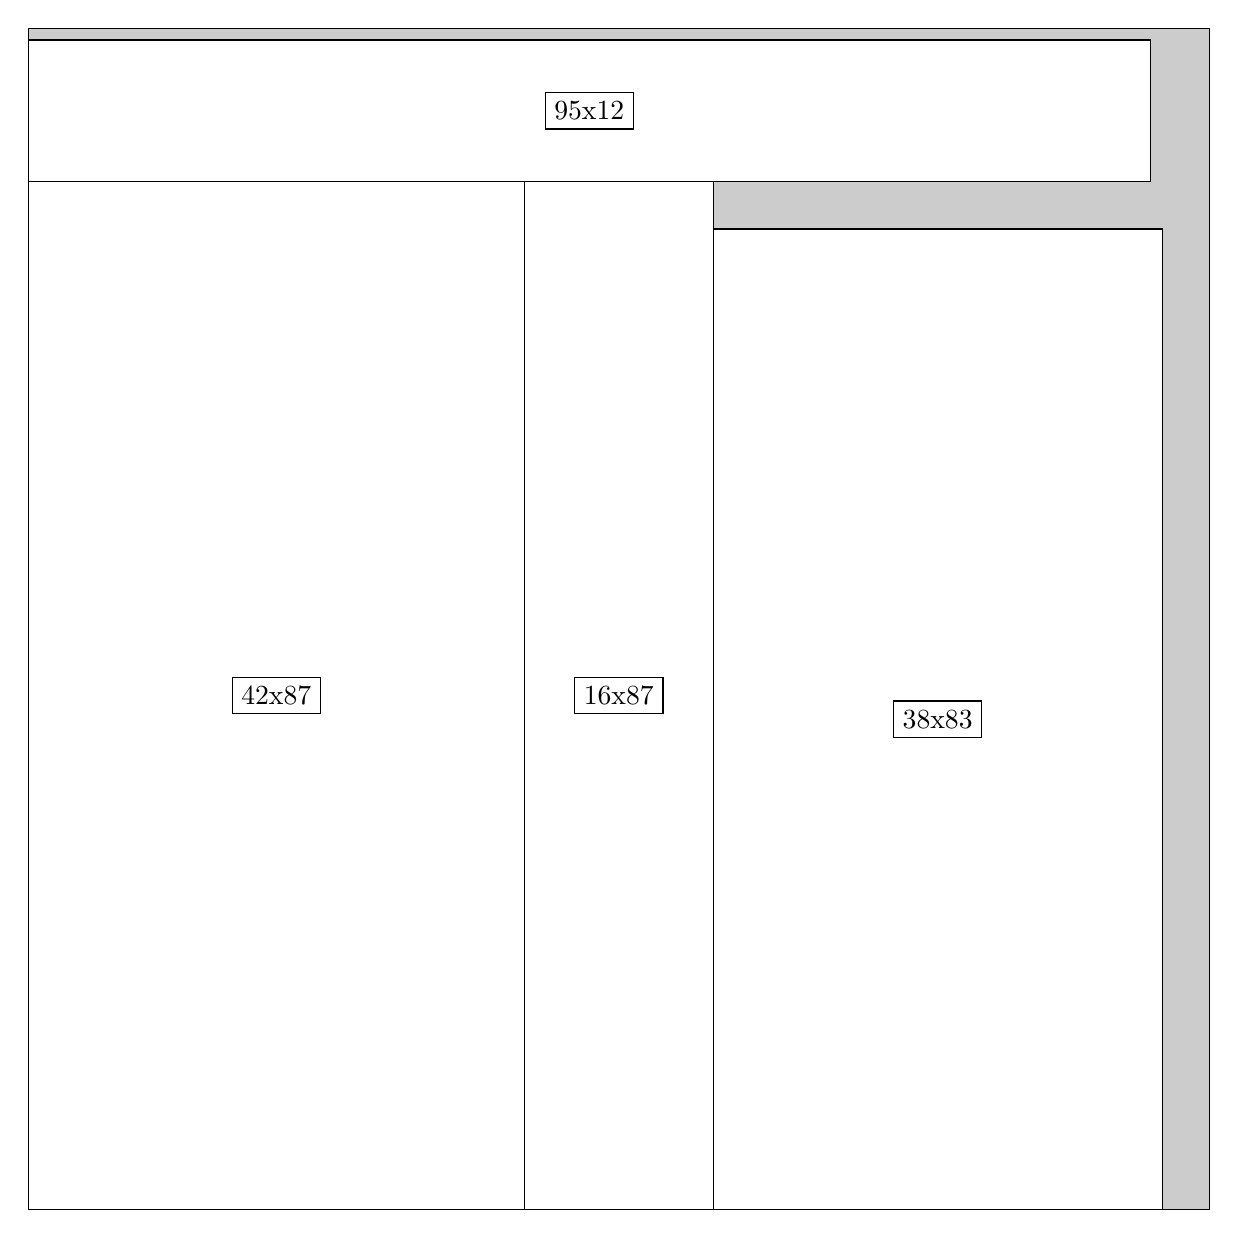
\begin{tikzpicture}[shorten >=1pt,scale=1.0,every node/.style={scale=1.0},->]
\tikzstyle{vertex}=[circle,fill=black!25,minimum size=14pt,inner sep=0pt]
\filldraw[fill=gray!40!white, draw=black] (0,0) rectangle (15.0,15.0);
\foreach \name/\x/\y/\w/\h in {42x87/0.0/0.0/6.3/13.049999999999999,38x83/8.7/0.0/5.7/12.45,16x87/6.3/0.0/2.4/13.049999999999999,95x12/0.0/13.049999999999999/14.25/1.7999999999999998}
\filldraw[fill=white!40!white, draw=black] (\x,\y) rectangle node[draw] (\name) {\name} ++(\w,\h);
\end{tikzpicture}


w =42 , h =87 , x =0 , y =0 , v =3654
\par
w =38 , h =83 , x =58 , y =0 , v =3154
\par
w =16 , h =87 , x =42 , y =0 , v =1392
\par
w =95 , h =12 , x =0 , y =87 , v =1140
\par
\newpage


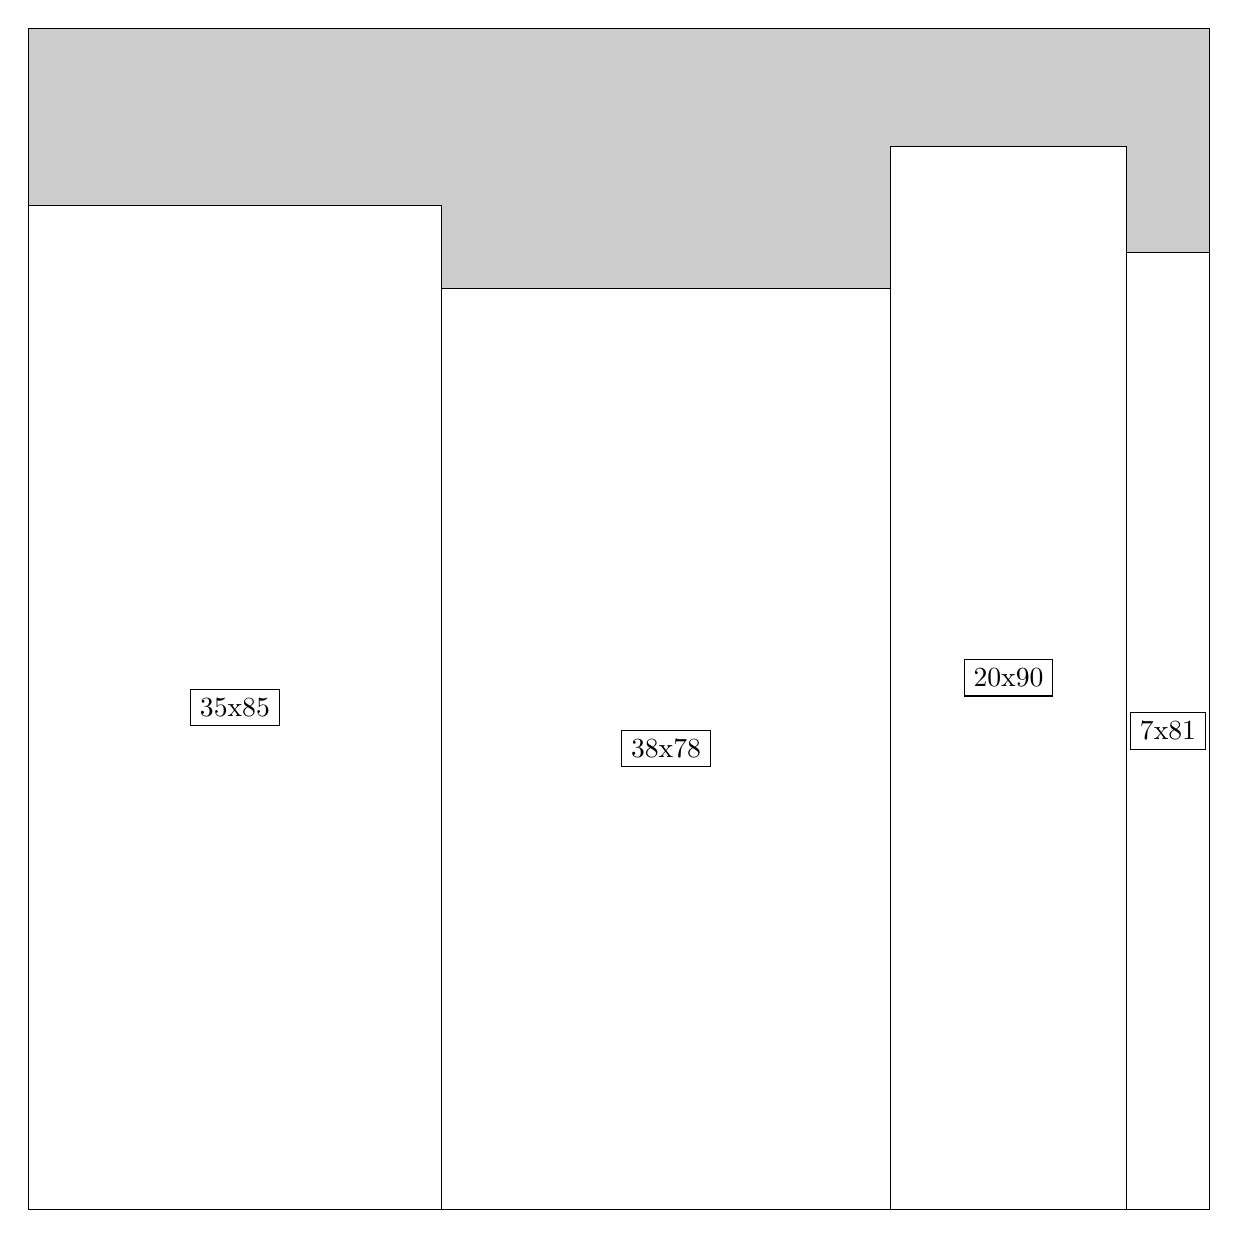
\begin{tikzpicture}[shorten >=1pt,scale=1.0,every node/.style={scale=1.0},->]
\tikzstyle{vertex}=[circle,fill=black!25,minimum size=14pt,inner sep=0pt]
\filldraw[fill=gray!40!white, draw=black] (0,0) rectangle (15.0,15.0);
\foreach \name/\x/\y/\w/\h in {35x85/0.0/0.0/5.25/12.75,38x78/5.25/0.0/5.7/11.7,20x90/10.95/0.0/3.0/13.5,7x81/13.95/0.0/1.05/12.15}
\filldraw[fill=white!40!white, draw=black] (\x,\y) rectangle node[draw] (\name) {\name} ++(\w,\h);
\end{tikzpicture}


w =35 , h =85 , x =0 , y =0 , v =2975
\par
w =38 , h =78 , x =35 , y =0 , v =2964
\par
w =20 , h =90 , x =73 , y =0 , v =1800
\par
w =7 , h =81 , x =93 , y =0 , v =567
\par
\newpage


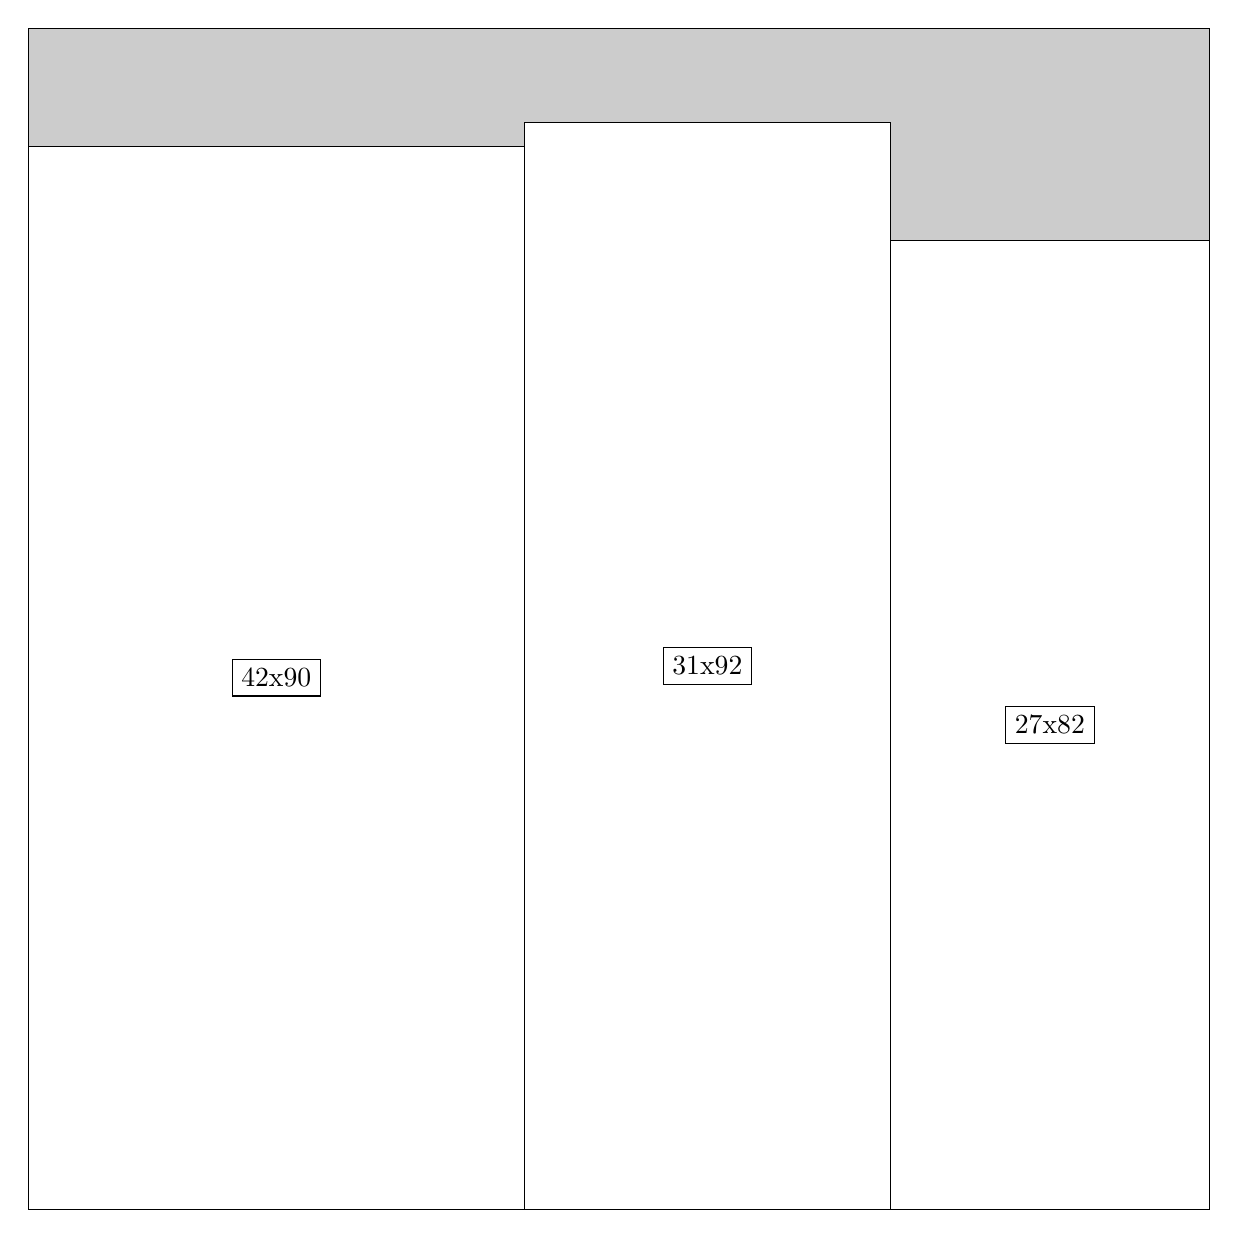
\begin{tikzpicture}[shorten >=1pt,scale=1.0,every node/.style={scale=1.0},->]
\tikzstyle{vertex}=[circle,fill=black!25,minimum size=14pt,inner sep=0pt]
\filldraw[fill=gray!40!white, draw=black] (0,0) rectangle (15.0,15.0);
\foreach \name/\x/\y/\w/\h in {42x90/0.0/0.0/6.3/13.5,31x92/6.3/0.0/4.6499999999999995/13.799999999999999,27x82/10.95/0.0/4.05/12.299999999999999}
\filldraw[fill=white!40!white, draw=black] (\x,\y) rectangle node[draw] (\name) {\name} ++(\w,\h);
\end{tikzpicture}


w =42 , h =90 , x =0 , y =0 , v =3780
\par
w =31 , h =92 , x =42 , y =0 , v =2852
\par
w =27 , h =82 , x =73 , y =0 , v =2214
\par
\newpage


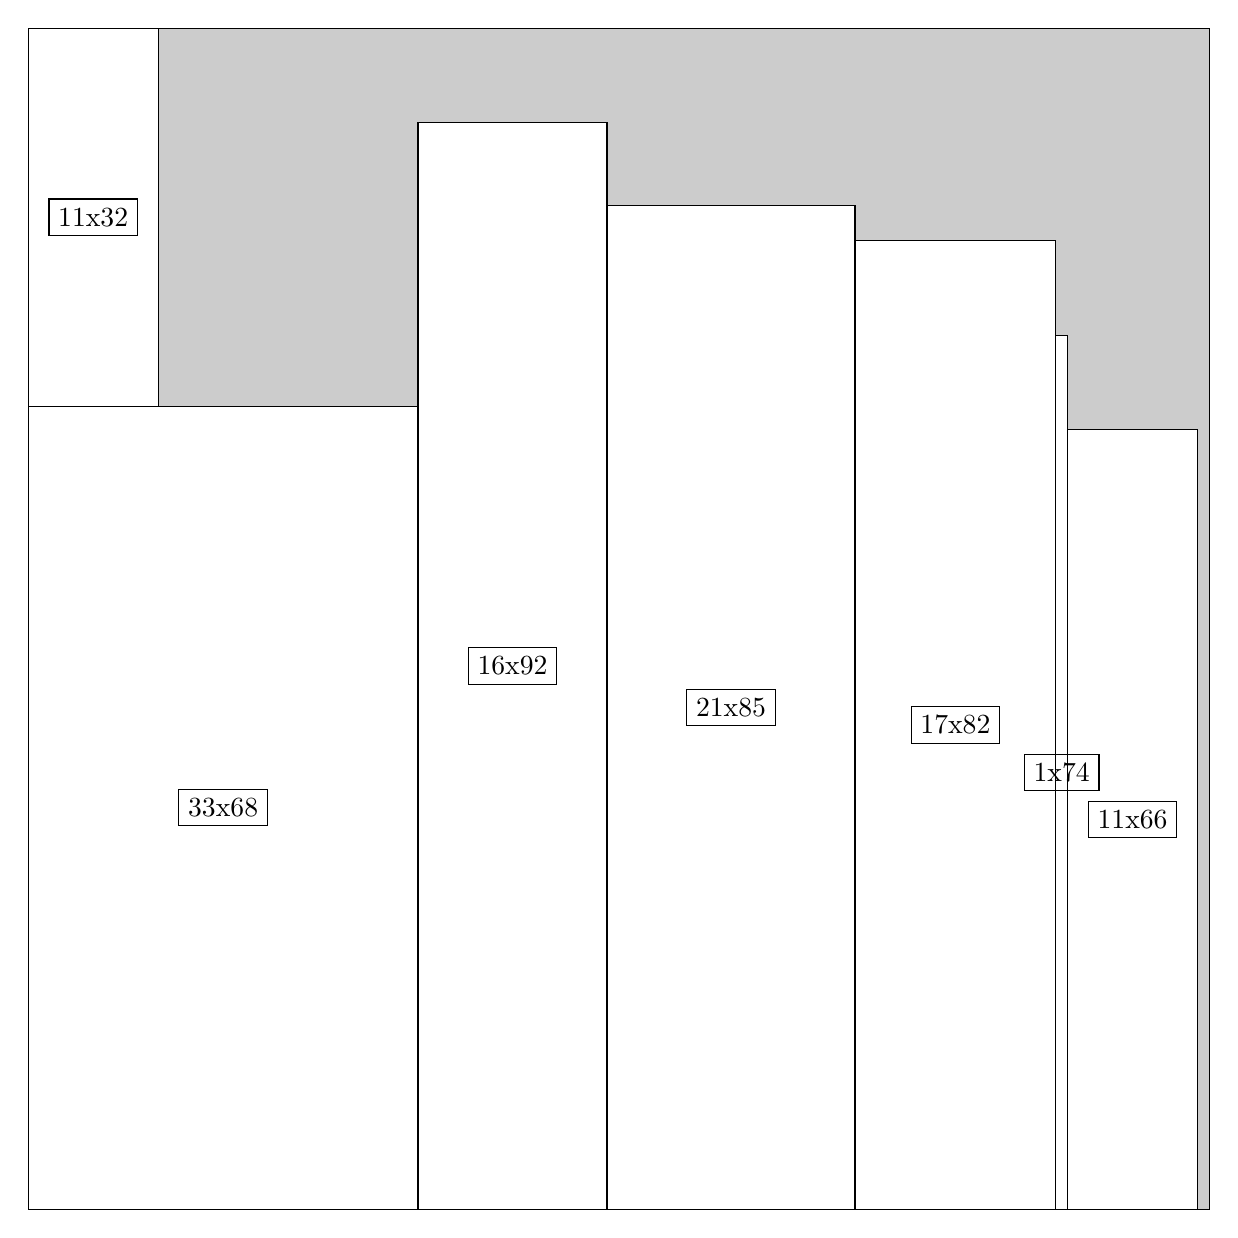
\begin{tikzpicture}[shorten >=1pt,scale=1.0,every node/.style={scale=1.0},->]
\tikzstyle{vertex}=[circle,fill=black!25,minimum size=14pt,inner sep=0pt]
\filldraw[fill=gray!40!white, draw=black] (0,0) rectangle (15.0,15.0);
\foreach \name/\x/\y/\w/\h in {33x68/0.0/0.0/4.95/10.2,21x85/7.35/0.0/3.15/12.75,16x92/4.95/0.0/2.4/13.799999999999999,17x82/10.5/0.0/2.55/12.299999999999999,11x66/13.2/0.0/1.65/9.9,11x32/0.0/10.2/1.65/4.8,1x74/13.049999999999999/0.0/0.15/11.1}
\filldraw[fill=white!40!white, draw=black] (\x,\y) rectangle node[draw] (\name) {\name} ++(\w,\h);
\end{tikzpicture}


w =33 , h =68 , x =0 , y =0 , v =2244
\par
w =21 , h =85 , x =49 , y =0 , v =1785
\par
w =16 , h =92 , x =33 , y =0 , v =1472
\par
w =17 , h =82 , x =70 , y =0 , v =1394
\par
w =11 , h =66 , x =88 , y =0 , v =726
\par
w =11 , h =32 , x =0 , y =68 , v =352
\par
w =1 , h =74 , x =87 , y =0 , v =74
\par
\newpage


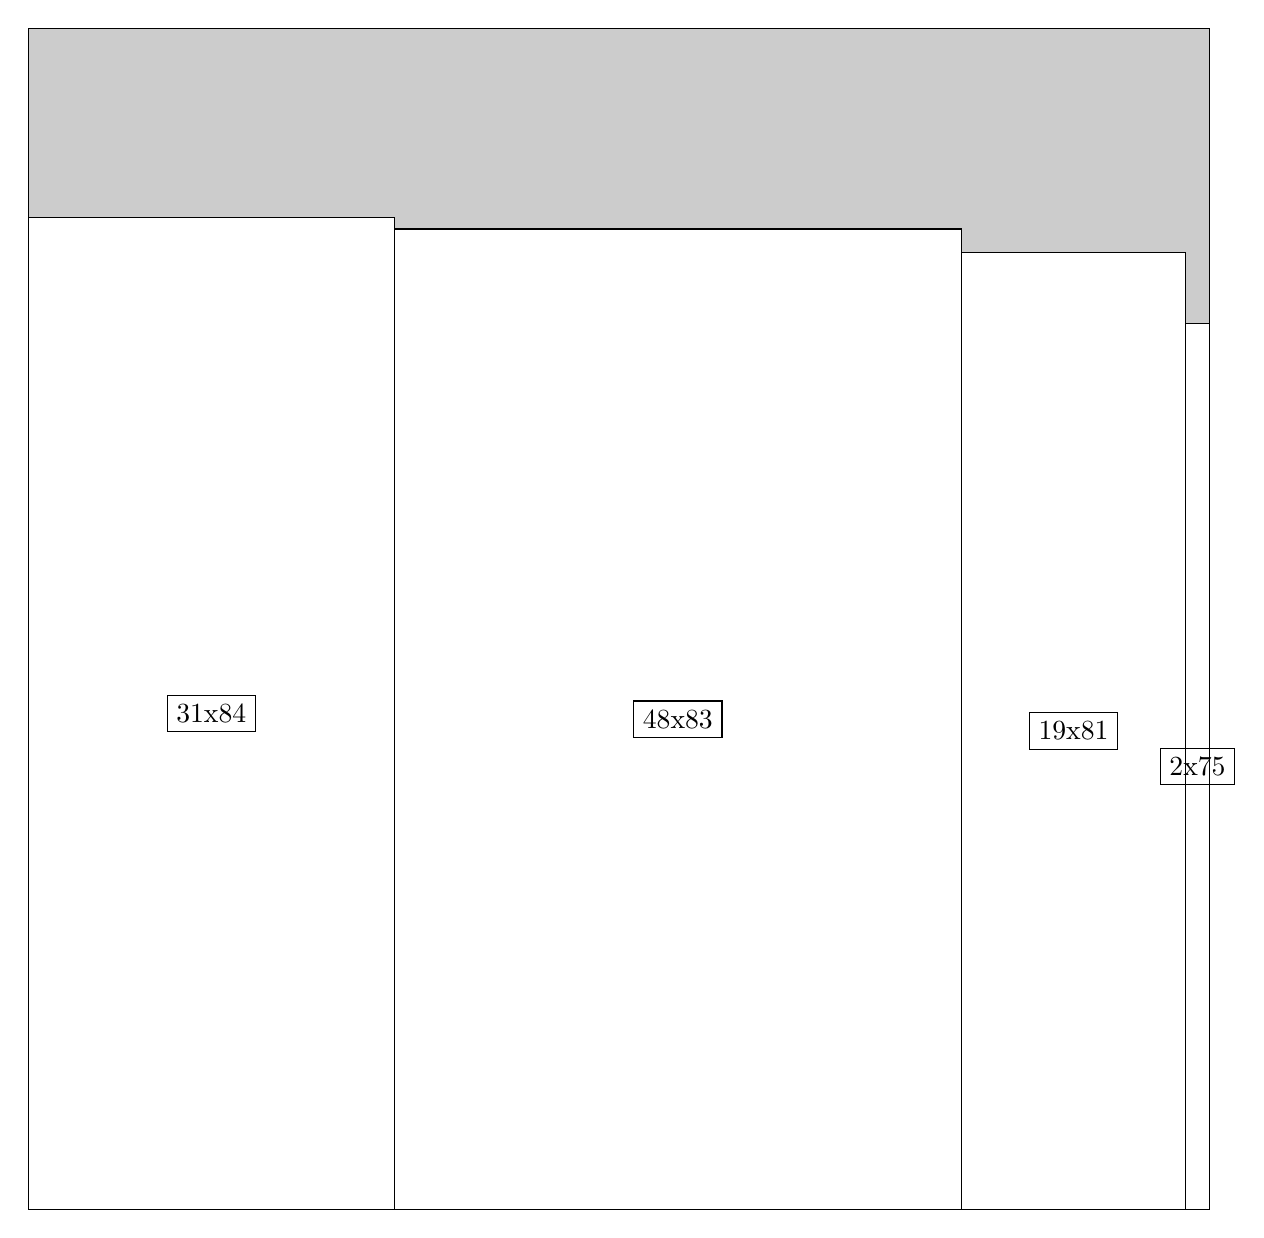
\begin{tikzpicture}[shorten >=1pt,scale=1.0,every node/.style={scale=1.0},->]
\tikzstyle{vertex}=[circle,fill=black!25,minimum size=14pt,inner sep=0pt]
\filldraw[fill=gray!40!white, draw=black] (0,0) rectangle (15.0,15.0);
\foreach \name/\x/\y/\w/\h in {48x83/4.6499999999999995/0.0/7.199999999999999/12.45,31x84/0.0/0.0/4.6499999999999995/12.6,19x81/11.85/0.0/2.85/12.15,2x75/14.7/0.0/0.3/11.25}
\filldraw[fill=white!40!white, draw=black] (\x,\y) rectangle node[draw] (\name) {\name} ++(\w,\h);
\end{tikzpicture}


w =48 , h =83 , x =31 , y =0 , v =3984
\par
w =31 , h =84 , x =0 , y =0 , v =2604
\par
w =19 , h =81 , x =79 , y =0 , v =1539
\par
w =2 , h =75 , x =98 , y =0 , v =150
\par
\newpage


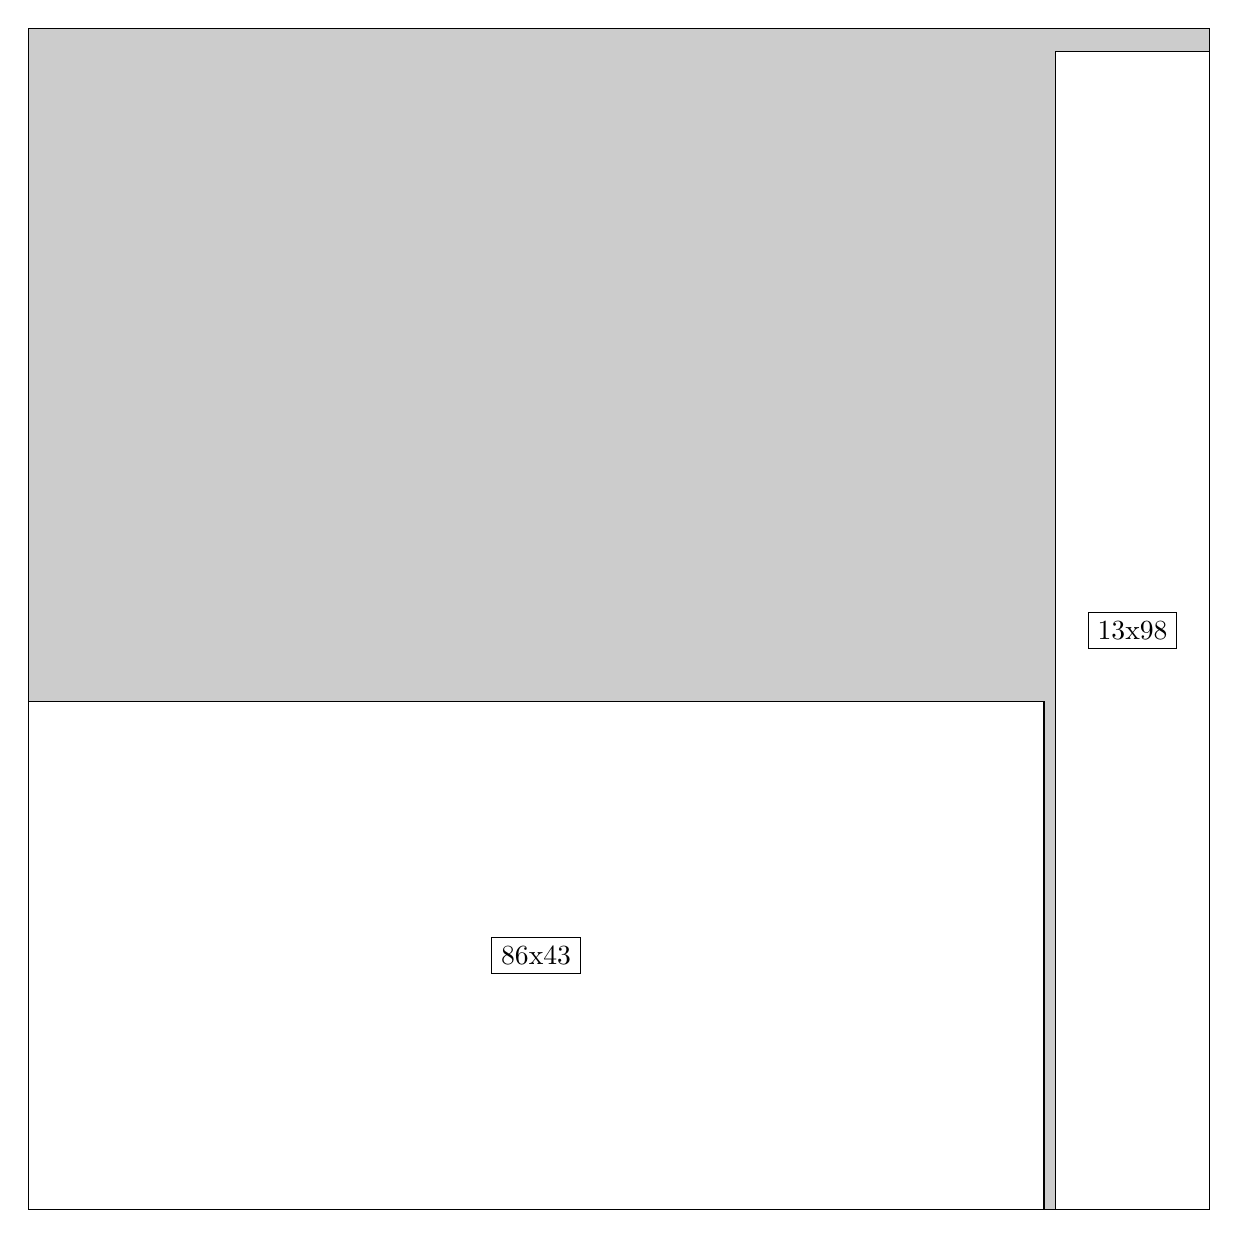
\begin{tikzpicture}[shorten >=1pt,scale=1.0,every node/.style={scale=1.0},->]
\tikzstyle{vertex}=[circle,fill=black!25,minimum size=14pt,inner sep=0pt]
\filldraw[fill=gray!40!white, draw=black] (0,0) rectangle (15.0,15.0);
\foreach \name/\x/\y/\w/\h in {86x43/0.0/0.0/12.9/6.45,13x98/13.049999999999999/0.0/1.95/14.7}
\filldraw[fill=white!40!white, draw=black] (\x,\y) rectangle node[draw] (\name) {\name} ++(\w,\h);
\end{tikzpicture}


w =86 , h =43 , x =0 , y =0 , v =3698
\par
w =13 , h =98 , x =87 , y =0 , v =1274
\par
\newpage


\end{document}